\documentclass[12pt,a4paper]{article}
\usepackage[utf8]{vietnam}
\usepackage[english]{babel} 
\usepackage{graphicx}
\usepackage{array}
\usepackage{booktabs}
\usepackage{amsmath}
\usepackage{hyperref}
\usepackage[left=2cm,right=2cm,top=2cm,bottom=2cm]{geometry}

\title{POSTS AND TELECOMMUNICATIONS INSTITUTE OF TECHNOLOGY\\
FACULTY OF INFORMATION TECHNOLOGY I\\
DEPARTMENT OF PYTHON PROGRAMMING}
\author{PYTHON PROGRAMMING REPORT}
\date{}

\begin{document}

\maketitle

\begin{center}
\includegraphics[width=1.4166666666666667in,height=1.84375in]{image1.png}
\end{center}

\begin{tabular}{ll}
\textbf{Lecturers of the Department} & : KIM NGỌC BÁCH \\
\textbf{Class} & : D23CQCE04 - B \\
\textbf{Student ID} & : B23DCCE076 \\
\textbf{Full name} & : NGUYỄN HỮU NIÊM \\
\end{tabular}

\newpage

\tableofcontents

\newpage

\section{Collecting Player Data from FBRef}

\subsection{Objective}
To collect statistical data for players who played more than 90 minutes in the 2024–2025 Premier League season from \url{https://fbref.com}.

\subsection{Methodology}

\subsubsection{Step 1: Identify Data Sources}
Data is collected from the following statistical tables on: https://fbref.com/en/comps/9/Premier-League-Stats
\begin{itemize}
\item Standard Stats
\item Goalkeeping
\item Shooting
\item Passing
\item GCA/SCA (Goal and Shot Creation)
\item Defense
\item Possession
\item Miscellaneous
\end{itemize}

\subsubsection{Step 2: Set Up Selenium}
The \texttt{webdriver\_manager} library is used to automatically download the compatible version of ChromeDriver.  
The browser runs in headless mode to optimize performance and avoid displaying a window during data collection.

\subsubsection{Step 3: Extract Data from Each Table}
\begin{verbatim}
def scrape_table_with_selenium(url, table_id):
    try:
        print(f"Scraping {url}...")
        driver.get(url)
        time.sleep(5)  # Increased wait time

        # Wait for table to load
        table = driver.find_element(By.ID, table_id)
        html = table.get_attribute('outerHTML')

        # Use StringIO to avoid the FutureWarning
        df = pd.read_html(StringIO(html))[0]

        # Clean multi-index columns
        if isinstance(df.columns, pd.MultiIndex):
            df.columns = ['_'.join(col).strip() for col in df.columns.values]

        # Standardize column names
        df.columns = df.columns.str.replace(r'%', 'pct', regex=True)
        df.columns = df.columns.str.replace(r'[^a-zA-Z0-9_]', '_', regex=True)

        return df

    except Exception as e:
        print(f"Error scraping {url}: {str(e)}")
        return None
    
\end{verbatim}

A function named \texttt{scrape\_table\_with\_selenium()} was built to:
\begin{itemize}
\item Navigate to each URL containing the statistical table
\item Locate the table using its HTML ID
\item Convert the HTML into a DataFrame using \texttt{pandas.read\_html()}
\item Clean column names (remove special characters, handle multi-index headers)
\end{itemize}

\subsubsection{Step 4: Clean and Merge Data}
\begin{itemize}
\item Normalize player and team names
\item Merge tables using \texttt{Player} and \texttt{Squad} columns with \texttt{pd.merge()}
\item Filter players with total minutes played > 90
\item Drop duplicate or unnecessary columns
\end{itemize}

\subsubsection{Step 5: Select and Rename Columns}
\begin{itemize}
\item Keep only the important statistical columns specified in the assignment
\item Rename unclear column names into readable and standardized forms such as \texttt{Goals}, \texttt{Assists}, \texttt{xG}, \texttt{Touches}, \texttt{Tackles}, etc.
\end{itemize}

\subsubsection{Step 6: Handle Missing Data and Format Values}
\begin{itemize}
\item Replace missing values with \texttt{"N/a"}
\item Normalize the nationality column to keep only country names instead of flag icons
\end{itemize}

\subsubsection{Step 7: Export the Data}
\begin{itemize}
\item Final cleaned data is exported to a file named \texttt{results.csv} for further analysis
\end{itemize}

\subsection{Tools and Data Processing Techniques Used}
The following tools and techniques were used during post-processing:

\begin{itemize}
    \item \textbf{Handling Missing Values} \\
    \textit{Tool:} \texttt{pandas.fillna()} \\
    \textit{Purpose:} Replace missing values with \texttt{"N/a"} for consistency and to avoid errors in later steps.

    \item \textbf{Column Name Normalization} \\
    \textit{Tool:} \texttt{pandas.DataFrame.columns.str.replace()} with regular expressions (regex) \\
    \textit{Purpose:} Remove special characters such as \texttt{\%}, \texttt{(}, \texttt{)}, make column names easier to use and understand.

    \item \textbf{Merging Data from Multiple Tables} \\
    \textit{Tool:} \texttt{pandas.merge()} \\
    \textit{Purpose:} Combine statistical tables using \texttt{Player} and \texttt{Squad} to create a unified dataset.

    \item \textbf{Filtering Data Based on Conditions} \\
    \textit{Tool:} \texttt{pandas.query()} or boolean filtering \\
    \textit{Purpose:} Keep only players with more than 90 minutes of playing time as required.

    \item \textbf{Normalizing Nationality Column} \\
    \textit{Tool:} \texttt{.str.split(' ').str[-1]} \\
    \textit{Purpose:} Remove flag emojis and retain only the country names (e.g., \texttt{Spain} $\rightarrow$ \texttt{Spain}).

    \item \textbf{Final Sorting and Cleaning} \\
    \textit{Tool:} \texttt{sort\_values()}, \texttt{reset\_index()}, \texttt{drop\_duplicates()} \\
    \textit{Purpose:} Sort by player names, remove duplicates, and finalize the cleaned dataset for analysis.
\end{itemize}

\subsection{Results}
The final dataset was successfully exported to \texttt{results.csv}.

\subsection{Remarks}
During the process of collecting and processing player statistics from \texttt{FBRef.com}, I noted the following:

\begin{enumerate}
    \item \textbf{Data Complexity:} \\
    The data on FBRef is split into multiple tables with different structures and column counts. Some tables have unclear column names (e.g., \texttt{Unnamed: ...}) or use multi-index headers, which adds complexity to processing.

    \item \textbf{Technical Challenges:} \\
    Since FBRef displays data using JavaScript, libraries like \texttt{requests} or \texttt{BeautifulSoup} alone are insufficient. Therefore, \texttt{Selenium} was used to simulate a real browser. Loading tables can sometimes be slow or unstable, so \texttt{time.sleep()} was added to ensure the table is fully loaded before scraping. Column name collisions during merging were handled with suffixes and by dropping unnecessary columns (e.g., columns with \texttt{\_drop} suffix).

    \item \textbf{Data Processing Techniques:} \\
    Column normalization is essential for easier manipulation, especially for statistical analysis or plotting. Filtering players based on playing time helps eliminate noise from low-appearance players, ensuring meaningful analysis.

    \item \textbf{Lessons Learned:} \\
    I learned how to combine multiple Python libraries (\texttt{Selenium + pandas}) to solve a real-world data problem. I also gained experience in cleaning and organizing messy data from various sources into a single dataset. Furthermore, I practiced dealing with missing data and building a robust data processing pipeline.
\end{enumerate}



\section{Statistical Analysis and Data Visualization}

\subsection{Objective}
Conduct descriptive statistical analysis and data visualization to explore trends, distributions, and performance of players and teams in the 2024–2025 Premier League season. Calculate mean, median, and standard deviation for technical indicators. At the same time, identify the most outstanding team based on average performance.

\subsection{Methodology}
The analysis is carried out through the following specific steps:

\begin{itemize}
    \item \textbf{Step 1: Find top 3 players for each statistic} \\
    Use a loop to iterate through each statistical column, find the top 3 and bottom 3 players with the highest and lowest values, along with team, nationality, and position information. The results are saved to the file \texttt{top\_3.txt} to support individual performance evaluation.

    \item \textbf{Step 2: Descriptive statistics by team} \\
    Calculate the mean, median, and standard deviation for each indicator, applied to each team and the entire league. The results are saved in the file \texttt{results2.csv} for inter-team comparison.

    \item \textbf{Step 3: Visualize data using Histogram charts} \\
    Plot histograms for several attacking (Goals, Assists, Goals per Shot) and defensive (Tackles, Interceptions, Blocks) indicators. Charts are displayed for the entire league and for each team to assess distribution and playing characteristics.

    \item \textbf{Step 4: Identify leading team for each indicator} \\
    Compute the average value of each statistic for every team and identify the team with the highest value. Results are saved to the file \texttt{best\_teams\_per\_statistic.csv}, allowing identification of top-performing teams in each aspect.

    \item \textbf{Step 5: Determine the best overall team based on positive metrics} \\
    Identify a group of positive indicators (e.g., goals, assists, accurate passes...), then count how many times each team leads these indicators. The team with the most positive statistics is considered the most effective overall.
\end{itemize}

\subsection{Tools and data processing techniques used}
\begin{itemize}
    \item \textbf{Top 3 player analysis:} using \texttt{pandas} and \texttt{numpy} to identify the best and worst performing players for each statistic.
    
    \item \textbf{Descriptive statistics calculation:} using \texttt{pandas.groupby()}, \texttt{mean()}, \texttt{median()}, and \texttt{std()} to analyze average performance and variation by team.
    
    \item \textbf{Data visualization:} using \texttt{matplotlib.pyplot.hist()} to show the distribution of metrics through charts, enabling easy comparison among players and teams.
    
    \item \textbf{Best team analysis:} using logical filtering techniques in \texttt{pandas} to determine teams that excel in multiple key performance metrics.
\end{itemize}

\subsection{Results}
The analysis results are exported to the following files:
\begin{itemize}
    \item \texttt{top\_3.txt}: List of top 3 and bottom 3 players for each indicator.
    \item \texttt{results2.csv}: Descriptive statistics table (mean, median, std) by team and for the entire league.
    \item \texttt{best\_teams\_per\_statistic.csv}: List of teams leading each technical indicator.
    \item \texttt{team\_rankings\_by\_positive\_stats.csv}: Ranking table of teams with the most positive indicators.
\end{itemize}

\subsection{Remarks}
The analysis reveals clear differences among teams in scoring ability, defense, and ball control. Histogram charts help detect skewed distributions, outliers, or clustering of statistics in a small group of players. Identifying teams that lead in multiple positive indicators provides an objective and comprehensive view of overall performance across clubs.



\section{Player Clustering using the K-means Algorithm}

\subsection{Objective}
This section aims to categorize players in the 2024–2025 Premier League into groups with similar technical characteristics and playing styles. Such clustering facilitates tactical analysis, player recruitment, and performance evaluation. It also enables a deeper understanding of player distribution and the emergence of specific archetypes such as defensive specialists, attackers, or ball controllers.

\subsection{Methodology}

\subsubsection{Step 1: Data Preprocessing}
\begin{itemize}
    \item Convert the \texttt{Age} column to float type for numerical processing.
    \item Remove descriptive columns including \texttt{Player}, \texttt{Nation}, \texttt{Squad}, and \texttt{Position}.
    \item Handle missing values using \texttt{SimpleImputer} with the mean strategy.
    \item Standardize all numerical features using \texttt{StandardScaler}.
\end{itemize}

\subsubsection{Step 2: Determining the Optimal Number of Clusters}
\begin{itemize}
    \item \textbf{Elbow Method:} Plot the Within-Cluster Sum of Squares (WCSS) to identify the “elbow point.”
    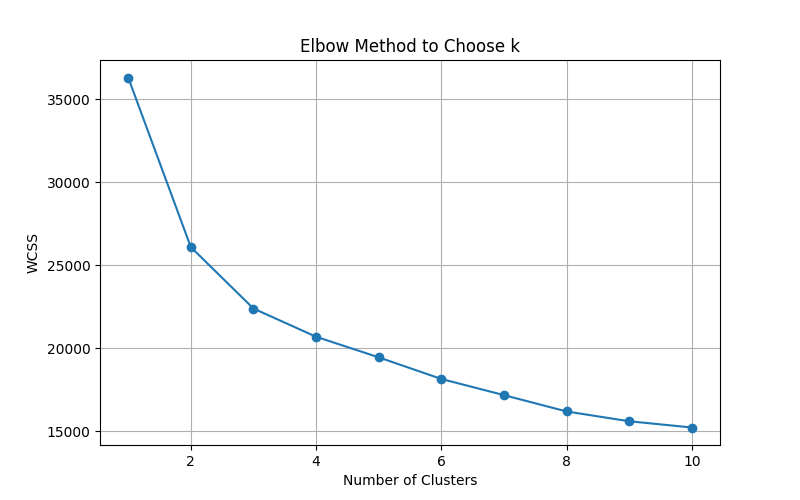
\includegraphics[width=2.8in,height=2in]{ProblemIII-elbow.png}
    \item \textbf{Silhouette Score:} Evaluate the quality of cluster separation for $k$ ranging from 2 to 10.
     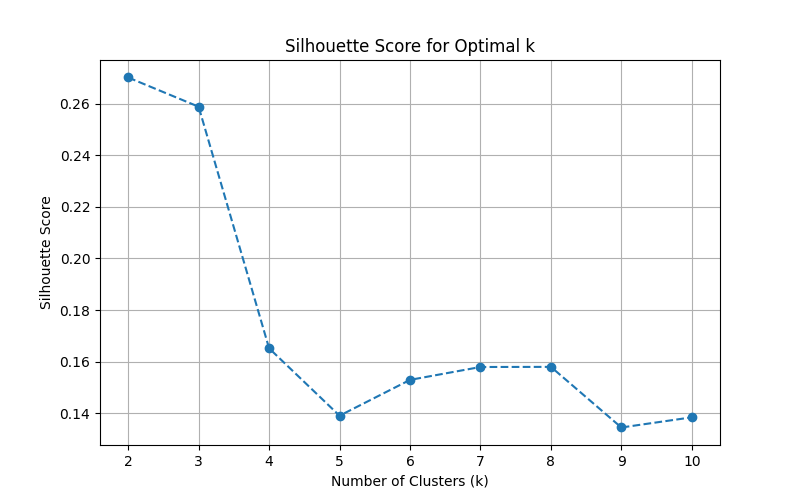
\includegraphics[width=2.8in,height=2in]{ProblemIII-Silhouette.png}
    \item Both methods indicate that $k = 8$ is the most appropriate number of clusters.
\end{itemize}

\subsubsection{Step 3: Applying the K-means Algorithm}
The \texttt{KMeans} algorithm is applied with $k = 8$ to segment the player dataset into 8 distinct clusters. Each player is assigned a corresponding cluster label, which is appended to the result dataset.

\subsubsection{Step 4: Cluster Profiling}
For each cluster, the mean of all technical indicators is computed to identify defining characteristics. Some example cluster archetypes include:
\begin{itemize}
    \item High goal-scoring cluster
    \item Defensive tackling cluster
    \item Ball control cluster
\end{itemize}

\subsubsection{Step 5: Visualizing Clustering Results with PCA}
\begin{itemize}
    \item Apply Principal Component Analysis (PCA) to reduce data dimensionality to 2D.
    \item Plot a scatter diagram with color-coded clusters.
    \item The visualization illustrates a clear separation between clusters in two-dimensional space.
\end{itemize}

\subsection{Tools and Libraries}
\begin{itemize}
    \item \textbf{scikit-learn:} Modules used include \texttt{KMeans}, \texttt{PCA}, \texttt{StandardScaler}, \texttt{SimpleImputer}, and \texttt{silhouette\_score}.
    \item \textbf{pandas:} For data manipulation and preparation.
    \item \textbf{matplotlib} and \textbf{seaborn:} For visual representation of clustering results.
\end{itemize}

\subsection{Results}
Clustering with $k = 8$ partitions players into eight distinct groups with unique technical profiles. The clusters reflect clearly different playing styles such as:
\begin{itemize}
    \item High goal scorers
    \item Creative playmakers
    \item Defensive disruptors
    \item Possession-oriented players
\end{itemize}
The PCA-based scatter plot confirms a well-defined separation of clusters in the 2D projection space.

\subsection{Discussion}
Clustering reveals common player archetypes within the league and supports practical applications such as transfer targeting, tactical squad building, and evaluating positional balance. However, the reliability of clustering results depends heavily on the selected features, and further validation using real-world match data is recommended.


\section{Player Value Prediction}

\subsection{Objective}
The objective of this section is to combine players' technical statistics with their estimated transfer values (ETV) to create a clean, complete dataset suitable for training machine learning models. This integration requires accurate player name matching, numerical data cleaning, and appropriate feature preparation for modeling.

\subsection{Methodology}

\subsubsection{Stage 1: Collecting and Normalizing ETV Data}
\begin{itemize}
    \item The \texttt{Selenium} library was used to automatically access 22 web pages from \texttt{footballtransfers.com}, each containing a list of Premier League players and their corresponding transfer values.
    \item HTML tables were located using Selenium methods to extract player names and ETVs.
    \item Player names were normalized by removing special characters, converting to lowercase, handling specific name cases (e.g., ``Son Heung-min'' to ``Heung Min Son''), and sorting name tokens for accurate matching.
    \item For players not found on the website or whose names could not be matched due to format differences, ETV values were manually assigned using a predefined mapping dictionary.
\end{itemize}

\subsubsection{Stage 2: Merging Technical Statistics with ETV Data}
\begin{itemize}
    \item Technical performance data was read from the \texttt{results.csv} file, containing detailed statistics such as goals, assists, tackles, etc.
    \item Data was merged using \texttt{pandas.merge()} based on normalized player names.
    \item An \texttt{inner} join strategy was applied to retain only players with both technical and ETV data.
    \item The merged dataset was saved as \texttt{results\_with\_etv.csv}.
\end{itemize}

\subsubsection{Stage 3: Cleaning and Preparing Training Data}
\begin{itemize}
    \item The \texttt{ETV} column (e.g., ``66.5M'') was converted to float by removing special characters.
\begin{verbatim}
df['ETV'] = df['ETV'].str.replace(r'[€M]', '', regex=True).astype(float)
df['ETV'] = np.clip(df['ETV'], df['ETV'].quantile(0.05), df['ETV'].quantile(0.95))
df['ETV'] = np.log1p(df['ETV'])
    
\end{verbatim}
    \item Clipping (5\% and 95\%) and log transformation (\texttt{log1p}) were applied to reduce the impact of outliers.
    \item The \texttt{Age} column was normalized from ``years-days'' format to a single float.
\begin{verbatim}
def convert_age(age):
    try:
        if isinstance(age, (int, float)):
            return float(age)
        if '-' in str(age):
            y, d = map(int, str(age).split('-'))
            return y + d / 365
        return float(age)
    except:
        return np.nan

df['Age'] = df['Age'].apply(convert_age)
df['Age'] = df['Age'].fillna(df['Age'].median()).round(1)
    
\end{verbatim}
    \item Remaining numerical features were cast to float and missing values were filled with zero.
    \item Irrelevant columns such as \texttt{Player}, \texttt{Nation}, \texttt{Squad}, and \texttt{Position} were removed.
\begin{verbatim}
def engineer_features(df):
    X = df.drop(columns=['ETV', 'Player', 'Nation', 'Squad'])
    y = df['ETV']
    if 'Position' in X.columns:
        X = X.drop(columns=['Position'])
    return X, y

X, y = engineer_features(df)
    
\end{verbatim}
    \item The dataset was split into training (80\%) and testing (20\%) sets using \texttt{train\_test\_split} from \texttt{scikit-learn}.
\end{itemize}


\subsubsection{Modeling and Evaluation}
Several machine learning models were trained to predict the log-transformed ETV values, including:
\begin{itemize}
    \item \textbf{Linear Regression}
    \item \textbf{Random Forest Regressor}
    \item \textbf{Gradient Boosting Regressor}
\end{itemize}

Among them, Gradient Boosting Regressor achieved the best results on the test set:
\begin{itemize}
    \item $R^2$: 0.6958
    \item RMSE: 0.4314
    \item MAE: 0.3451
    \item Spearman Rank Correlation: 0.7955
\end{itemize}

Feature importance was also extracted to understand the most influential attributes in player valuation.


\subsection{Tools and Libraries Used}
\begin{itemize}
    \item \textbf{Selenium}: For web scraping ETV data.
    \item \textbf{pandas}: For data processing, cleaning, and merging.
    \item \textbf{numpy}: For numerical transformations.
    \item \textbf{fuzzywuzzy}: For accurate player name matching.
    \item \textbf{regex}: For string formatting and cleaning.
    \item \textbf{scikit-learn}: For data preprocessing, splitting, and modeling support.
\end{itemize}

\subsection{Results}
The \texttt{results\_with\_etv.csv} dataset was successfully created, containing over 200 Premier League players with full information on nationality, age, club, position, and more than 50 technical performance indicators. ETV values were integrated and the dataset is ready for machine learning tasks.

\subsection{Discussion}
The integration phase was crucial since improper name normalization could result in mismatches or missing data. The log transformation of ETV values helped stabilize the data distribution and reduce the risk of model overfitting.

\section{Conclusions and Development Directions}

\subsection{Summary of the Implementation Process}
The project successfully developed a system for analyzing and estimating the value of Premier League players based on technical performance data and estimated transfer value (ETV). The implementation process included the following main stages:
\begin{itemize}
    \item Collected player technical statistics from FBRef.com using Selenium.
    \item Cleaned and integrated multiple statistical tables into a single aggregated dataset.
    \item Collected and standardized ETV data from footballtransfers.com.
    \item Merged the technical and ETV data to form a complete training dataset.
    \item Built machine learning models for player value prediction using algorithms such as Linear Regression, Random Forest, and Gradient Boosting.
\end{itemize}

\subsection{Model Efficiency and Achieved Results}
\begin{tabular}{|l|c|c|c|c|}
\hline
\textbf{Model} & \textbf{R²} & \textbf{RMSE} & \textbf{MAE} & \textbf{Spearman} \\
\hline
Linear Regression & 0.594  & 0.4948 & 0.4137 &  0.7846  \\
Random Forest     & 0.6661 & 0.4520 & 0.3512  & 0.7497  \\
Gradient Boosting & \textbf{0.6958} & \textbf{0.4314} & \textbf{0.3451} & \textbf{0.7955} \\
\hline
\end{tabular}

Among the models implemented, the Gradient Boosting Regressor yielded the best performance on the test set with the following metrics:
\begin{itemize}
    \item $R^2 = 0.6958$
    \item RMSE = 0.4314
    \item MAE = 0.3451
    \item Spearman correlation = 0.7955
\end{itemize}
These results indicate that the model can predict player values with relatively high accuracy, especially in ranking players by their market value.

\subsection{Highlights in the Implementation Process}
\begin{itemize}
    \item Successfully integrated data from multiple heterogeneous sources.
    \item Standardized player names to handle formatting inconsistencies during data merging.
    \item Applied preprocessing techniques such as outlier handling, log transformation, and normalization.
    \item Deployed a complete machine learning pipeline with automatic feature selection using Recursive Feature Elimination (RFE) to improve predictive performance.
\end{itemize}

\subsection{Limitations}
\begin{itemize}
    \item ETV data is time-sensitive but was collected at a single point in time.
    \item Some players were manually assigned ETV values due to missing data, which may cause minor inconsistencies.
    \item Certain potentially useful features such as tactical roles, recent performance trends, or team-related parameters were not deeply exploited.
\end{itemize}

\subsection{Future Development Directions}
\begin{itemize}
    \item Expand the model across multiple seasons to improve generalizability.
    \item Add more contextual features from the transfer market, such as player age, rarity of nationality, or contract duration.
    \item Deploy a web application or interactive dashboard that allows users to input player data and receive real-time ETV predictions.
    \item Experiment with advanced models such as XGBoost, LightGBM, or deep learning approaches.
\end{itemize}


\section*{Appendix}

\subsection*{A. Data Sources}
\begin{itemize}
    \item Player statistics: \url{https://fbref.com/en/comps/9/Premier-League-Stats}
    \item Estimated Transfer Values (ETV): \url{https://www.footballtransfers.com}
\end{itemize}

\subsection*{B. Key Technical Features Used}
\begin{itemize}
    \item Offensive: Goals, Assists, Expected Goals (xG), Shots on Target, xG per 90 minutes
    \item Defensive: Tackles, Interceptions, Blocks, Clearances
    \item Possession: Touches, Carries, Progressive Carries, Passing Accuracy
    \item Others: Minutes Played, Age (normalized), Positions (encoded)
\end{itemize}

\subsection*{C. Model Performance Summary}
\begin{center}
\begin{tabular}{lcccc}
\toprule
\textbf{Model} & \textbf{R\textsuperscript{2}} & \textbf{RMSE} & \textbf{MAE} & \textbf{Spearman} \\
\midrule
Linear Regression & 0.5940 & 0.4984 & 0.4137 & 0.7846 \\
Random Forest     & 0.6661 & 0.4520 & 0.3512 & 0.7497 \\
Gradient Boosting & \textbf{0.6958} & \textbf{0.4314} & \textbf{0.3451} & \textbf{0.7955} \\
\bottomrule
\end{tabular}
\end{center}

\subsection*{D. Tools and Libraries}
\begin{itemize}
    \item \textbf{Selenium} – Web scraping from dynamic websites
    \item \textbf{pandas, numpy} – Data manipulation and numerical computation
    \item \textbf{scikit-learn} – Machine learning models, preprocessing, evaluation
    \item \textbf{fuzzywuzzy} – Fuzzy string matching for player name alignment
    \item \textbf{matplotlib, seaborn} – Data visualization
\end{itemize}

\newpage
\section*{References}

\begin{itemize}
    \item FBRef. Premier League Player Stats. \url{https://fbref.com/en/comps/9/Premier-League-Stats}
    \item FootballTransfers. Estimated Transfer Values. \url{https://www.footballtransfers.com}
    \item scikit-learn: Machine Learning in Python. \url{https://scikit-learn.org/stable/}
    \item pandas Documentation. \url{https://pandas.pydata.org/}
    \item Selenium Python Docs. \url{https://selenium-python.readthedocs.io/}
    \item matplotlib Documentation. \url{https://matplotlib.org/}
    \item seaborn Documentation. \url{https://seaborn.pydata.org/}
\end{itemize}



\end{document}
